% Options for packages loaded elsewhere
\PassOptionsToPackage{unicode}{hyperref}
\PassOptionsToPackage{hyphens}{url}
\documentclass[
  11pt,
]{article}
\usepackage{xcolor}
\usepackage[margin=22mm]{geometry}
\usepackage{amsmath,amssymb}
\setcounter{secnumdepth}{-\maxdimen} % remove section numbering
\usepackage{iftex}
\ifPDFTeX
  \usepackage[T1]{fontenc}
  \usepackage[utf8]{inputenc}
  \usepackage{textcomp} % provide euro and other symbols
\else % if luatex or xetex
  \usepackage{unicode-math} % this also loads fontspec
  \defaultfontfeatures{Scale=MatchLowercase}
  \defaultfontfeatures[\rmfamily]{Ligatures=TeX,Scale=1}
\fi
\usepackage{lmodern}
\ifPDFTeX\else
  % xetex/luatex font selection
\fi
% Use upquote if available, for straight quotes in verbatim environments
\IfFileExists{upquote.sty}{\usepackage{upquote}}{}
\IfFileExists{microtype.sty}{% use microtype if available
  \usepackage[]{microtype}
  \UseMicrotypeSet[protrusion]{basicmath} % disable protrusion for tt fonts
}{}
\makeatletter
\@ifundefined{KOMAClassName}{% if non-KOMA class
  \IfFileExists{parskip.sty}{%
    \usepackage{parskip}
  }{% else
    \setlength{\parindent}{0pt}
    \setlength{\parskip}{6pt plus 2pt minus 1pt}}
}{% if KOMA class
  \KOMAoptions{parskip=half}}
\makeatother
\setlength{\emergencystretch}{3em} % prevent overfull lines
\providecommand{\tightlist}{%
  \setlength{\itemsep}{0pt}\setlength{\parskip}{0pt}}
\usepackage{bookmark}
\IfFileExists{xurl.sty}{\usepackage{xurl}}{} % add URL line breaks if available
\urlstyle{same}
\hypersetup{
  hidelinks,
  pdfcreator={LaTeX via pandoc}}

\author{}
\date{}

\usepackage{graphicx}
\begin{document}

\section{Exact reflection and phase transport for the original
operator}\label{exact-reflection-and-phase-transport-for-the-original-operator}

This separate reflection and adjoint supplement proves an exact
transport for the original operator. Its complete graph-domain
foundations are in
\href{../u006-graph-domains/graph-domain-note.html}{The two graph-domain
quotients of the local inverse}. The receiving original-source proofs
are
\href{https://github.com/KokunoYumeto/open-math-courses/blob/b1f73325069d9568d9acb6e27036b1b0f4cad7fd/docs/courses/elliptic-operators-and-boundary-problems/src/local-elliptic-coefficients.md\#L1846}{Local
inverse, Section 14.6, (CS40)--(CS50)} and
\href{https://github.com/KokunoYumeto/open-math-courses/blob/b1f73325069d9568d9acb6e27036b1b0f4cad7fd/docs/courses/elliptic-operators-and-boundary-problems/src/local-elliptic-coefficients.md\#L2218}{Section
14.8.5, (CE25)--(CE34)}. The complete packaged proofs are
\href{../../local-elliptic-coefficients.html\#eq-CS40}{the local inverse
identities} and
\href{../../local-elliptic-coefficients.html\#eq-CE25}{the
original-coefficient example}. The pinned source citations require
repository access. No new external theorem is used, and no novelty is
claimed.

All Hilbert inner products below are linear in their first argument.
Distribution pairings are complex bilinear. The resulting distinction
between the Hilbert adjoint and distributional transpose is retained
explicitly.

\subsection{1. Fixed quantities and the involution on functions and
distributions}\label{fixed-quantities-and-the-involution-on-functions-and-distributions}

Keep the original coordinates and all constants:

\[
 U=(-1/4,1/4)^2,\qquad D_j=-i\partial_{x_j},\qquad
 p(\xi_1,\xi_2)=\xi_1^2+i\xi_2,
\] \[
 C=\begin{pmatrix}14&-20&7\\-20&32&-12\\7&-12&5\end{pmatrix},
 \quad\lambda_*=\text{the largest eigenvalue of }C,\quad
 K=41472\lambda_*\sqrt{33}\,e^2,\quad
 a=\sqrt{\frac{\sqrt2-1}{2}},\quad
 \varepsilon=\frac2{Ka}>0 .
 \tag{JM1}
\]

Let \(Y=L^2(U)\). For every polynomial
\(q\), keep its complete derivative strength
\[
 \widetilde q(\xi)^2=\sum_{\alpha\in\mathbb N^2}
                              |\partial_\xi^\alpha q(\xi)|^2,
 \quad
 V_p=\{q:\sup_{\xi\in\mathbb R^2}\widetilde q(\xi)/\widetilde p(\xi)<\infty\},
 \quad
 \|q\|_p=\sup_{\xi\in\mathbb R^2}\frac{\widetilde q(\xi)}{\widetilde p(\xi)}.
\] For any actual declared basis
\(q_1,\ldots,q_4\) of the exact space \(V_p\),
define \[
 H=\{u\in L^2(U):q_j(D)u\in L^2(U),\ 1\leq j\leq4\},
 \quad
 \|u\|_H^2=\|u\|_2^2+\sum_{j=1}^4\|q_j(D)u\|_2^2,
 \quad H_{\min}=\overline{C_c^\infty(U)}^{\|\cdot\|_H}.
 \tag{JM2}
\] The complete proofs of finite dimension,
Hilbert completeness, \(V_p=\operatorname{span}\{1,\xi_1,\xi_1^2,\xi_2\}\), and the four monomial
norms are
\href{../u006-graph-domains/graph-domain-note.html\#eq-GM1}{GM1}--\href{../u006-graph-domains/graph-domain-note.html\#eq-GM2}{GM2}
and \href{../u006-graph-domains/graph-domain-note.html\#eq-GM31}{GM31}
of the retained note. No norm for a different basis is substituted for
(JM2).

Retain the original full operator and its full Hilbert formal adjoint:
\[
 P=D_1^2+iD_2+\varepsilon x_1D_1
    =-\partial_1^2+\partial_2-i\varepsilon x_1\partial_1,
\] \[
 A=P^\dagger
    =D_1^2-iD_2+\varepsilon x_1D_1-i\varepsilon
    =-\partial_1^2-\partial_2-i\varepsilon x_1\partial_1-i\varepsilon.
 \tag{JM3}
\] The zeroth-order term is
the contribution from \(D_1(\varepsilon x_1 v)=\varepsilon x_1D_1v-i\varepsilon v\). It is retained in every
calculation below. For this specific smooth coefficient, both
expressions act on every distribution; this does not assert that an
arbitrary continuous coefficient can multiply any distributional
derivative.

Put \[
 \rho(x_1,x_2)=(x_1,-x_2),\qquad
 Jf(x_1,x_2)=e^{-i\varepsilon x_2}f(x_1,-x_2).
 \tag{JM4}
\] The real reflection has determinant
\(-1\), absolute Jacobian \(1\), and
preserves the actual open square. Since \(\varepsilon\) is real,
its displayed phase has modulus one. Thus change of variables, with
Lebesgue measure and the absolute Jacobian retained, gives
\[
 \langle Jf,Jh\rangle_2
   =\int_U e^{-i\varepsilon x_2}f(x_1,-x_2)
                    e^{i\varepsilon x_2}\overline{h(x_1,-x_2)}\,dx_1\,dx_2
   =\langle f,h\rangle_2 .
\] Applying the exact phase twice gives
\[
 J^2f(x)
   =e^{-i\varepsilon x_2}e^{-i\varepsilon(-x_2)}f(x)=f(x),
 \qquad \|Jf\|_2=\|f\|_2,\qquad J^*=J .
 \tag{JM5}
\] Consequently \(J\) is a
complex-linear unitary involution on \(Y\).

Its distributional extension is specified by the actual bilinear
transpose: \[
 \langle JT,\phi\rangle_{\mathcal D',\mathcal D}
    =\langle T,J^{\mathrm t}\phi\rangle_{\mathcal D',\mathcal D},
 \qquad
 J^{\mathrm t}\phi(x_1,x_2)
      =e^{i\varepsilon x_2}\phi(x_1,-x_2).
 \tag{JM6}
\] The test transform maps
\(C_c^\infty(U)\) continuously to itself; reflection preserves
compact support, and differentiation of its smooth phase leaves a finite
sum of smooth bounded factors on each compact set. Formula (JM6)
therefore defines a distribution for every \(T\). For
an \(L^2\) function, the substitution
\(x_2\mapsto-x_2\) in its bilinear integral gives precisely this
formula, so it agrees with (JM4). The test transform also squares to the
identity, because its phases are \(e^{i\varepsilon x_2}\) and
\(e^{-i\varepsilon x_2}\). Thus \(J^2=I\) on distributions.
In particular the plus sign in \(J^{\mathrm t}\) is not replaced
by the minus sign of the function formula or by the Hilbert adjoint
convention.

For smooth functions, differentiation retains the complete phase
contributions and gives \[
 D_1J=JD_1,\qquad
 D_2J=J(-D_2-\varepsilon),\qquad
 x_1J=Jx_1 .
 \tag{JM7}
\] Indeed differentiation
of \(e^{-i\varepsilon x_2}\) contributes \((-i)(-i\varepsilon)e^{-i\varepsilon x_2}=-\varepsilon e^{-i\varepsilon x_2}\);
differentiation of the reflected argument contributes
\(i e^{-i\varepsilon x_2}(\partial_2f)(x_1,-x_2)\). Together these are exactly the second formula.
The other coordinate and multiplication formulas follow because neither
its phase nor its reflection changes \(x_1\).

These formulas also hold on all distributions, without a regularity
premise. In the bilinear convention \(D_j^{\mathrm t}=-D_j\). On tests,
direct differentiation of the plus-phase transform gives
\(D_1J^{\mathrm t}=J^{\mathrm t}D_1\) and \(D_2J^{\mathrm t}=J^{\mathrm t}(-D_2+\varepsilon)\). For the second
distributional identity, pair its left side against
\(\phi\) to obtain \(\langle T,J^{\mathrm t}(-D_2\phi)\rangle\). The right
side pairs as \(\langle T,(D_2-\varepsilon)J^{\mathrm t}\phi\rangle\), which is the same expression by
the displayed test identity. The first and multiplication identities
follow by the same transpose calculation. Thus no differentiation or
coefficient term is lost in their distributional extension.

\subsection{2. The full weaker-polynomial pullback and every basis graph
bound}\label{the-full-weaker-polynomial-pullback-and-every-basis-graph-bound}

Define the original affine frequency transform \[
 \tau(\xi_1,\xi_2)=(\xi_1,-\xi_2-\varepsilon),\qquad
 q^\#(\xi)=q(\xi_1,-\xi_2-\varepsilon).
\]
It is an involution. Applying (JM7) successively to each monomial, then
adding every coefficient, gives on all distributions
\[
 q(D)J=Jq^\#(D),\qquad
 \partial_\xi^\alpha q^\#(\xi)
       =(-1)^{\alpha_2}(\partial_\xi^\alpha q)(\tau\xi),
 \qquad
 \widetilde{q^\#}(\xi)=\widetilde q(\tau\xi).
 \tag{JM8}
\] The chain rule has no additional higher-order
term, because \(\tau\) is affine with linear part
\(\operatorname{diag}(1,-1)\). Iterating the first-order chain rule proves the
sign \((-1)^{\alpha_2}\) for every multi-index, including zero
derivatives.

The full original \(p\)-strength at the reflected and
translated frequency is \[
 \widetilde p(\tau\xi)^2
    =\xi_1^4+(\xi_2+\varepsilon)^2+4\xi_1^2+1+4.
 \tag{JM9}
\] This contains the
nonzero translated-frequency contribution and both separate constants
\(1\) and \(4\). To compare it with
the original array, the complete derivative array of
\(p^\#=\xi_1^2-i\xi_2-i\varepsilon\) is the array of \(\overline p=\xi_1^2-i\xi_2\) with the
additional zeroth entry \(-i\varepsilon\) and no additional
derivative entries. The two arrays have exactly the same first and
second derivative entries and all the same zeros. The Euclidean triangle
inequality therefore gives \[
 \widetilde p(\tau\xi)\leq\widetilde p(\xi)+\varepsilon
       \leq\left(1+\frac{\varepsilon}{\sqrt5}\right)\widetilde p(\xi),
 \qquad \widetilde p(\xi)\geq\sqrt{1+4}=\sqrt5 .
\] For
\(q\in V_p\), keep every factor in \[
 \widetilde{q^\#}(\xi)
       =\widetilde q(\tau\xi)
       \leq\|q\|_p\,\widetilde p(\tau\xi)
       \leq\left(1+\frac{\varepsilon}{\sqrt5}\right)
                  \|q\|_p\,\widetilde p(\xi).
 \tag{JM10}
\]
Thus \(q^\#\in V_p\), with the exact proved bound
\(\|q^\#\|_p\leq(1+\varepsilon/\sqrt5)\|q\|_p\). Applying it again to \(q^\#\)
yields \(\|q\|_p\leq(1+\varepsilon/\sqrt5)\|q^\#\|_p\), because \((q^\#)^\#=q\). This
proves both directions of the comparison while retaining the original
polynomial as the receiving object.

Let the column of original monomials be \(r=(1,\xi_1,\xi_1^2,\xi_2)^{\mathrm T}\). For the
actual basis in (JM2), write its exact coefficient matrix as
\(q=B_0r\), where \(B_0\in\operatorname{GL}_4(\mathbb C)\). No coefficient
of this basis matrix is discarded. The pullback has the full matrices
\[
 r^\#=B_\#r,\qquad
 B_\#=
 \begin{pmatrix}
 1&0&0&0\\
 0&1&0&0\\
 0&0&1&0\\
 -\varepsilon&0&0&-1
 \end{pmatrix},\qquad
 q^\#=\beta q,\qquad
 \beta=B_0B_\#B_0^{-1},\qquad \beta^2=I_4 .
 \tag{JM11}
\] The last row retains the translation term
\(-\varepsilon\). The other zero entries are retained in the
printed matrix. The basis formula follows by inserting
\(r^\#\) into \(q^\#=B_0r^\#\). The involution
formula follows either by multiplying \(B_\#^2=I_4\) or by
applying the polynomial involution twice.

For \(u\in H\), (JM8) and (JM11) give
\(q_j(D)Ju=J\sum_k\beta_{jk}q_k(D)u\). Every right side is an \(L^2\)
function, which proves \(Ju\in H\). Exact
\(L^2\) unitarity then gives the original-norm identity
\[
 \|Ju\|_H^2
    =\|u\|_2^2
       +\sum_{j=1}^4
             \left\|\sum_{k=1}^4\beta_{jk}q_k(D)u\right\|_2^2.
 \tag{JM12}
\] Put \(\sigma_\beta=\|\beta\|_{\mathbb C^4\to\mathbb C^4}\), with the ordinary
Euclidean coefficient-vector norm, and \(\kappa_\beta=\max\{1,\sigma_\beta\}\). The
definition of this finite matrix norm and integration imply
\[
 \kappa_\beta^{-1}\|u\|_H
       \leq\|Ju\|_H\leq\kappa_\beta\|u\|_H,
 \qquad J:H\longrightarrow H\text{ is a bounded involution.}
 \tag{JM13}
\] The upper estimate uses (JM12) and its unchanged
separate \(L^2\) term. Apply it to
\(Ju\) and use \(J^2u=u\) for the lower
estimate. If a directly summed finite bound is desired,
\(\sigma_\beta\leq(\sum_{j,k}|\beta_{jk}|^2)^{1/2}\) follows by rowwise Cauchy--Schwarz; every actual
basis coefficient remains in that sum.

For the declared monomial basis of
\href{../u006-graph-domains/graph-domain-note.html\#eq-GM32}{GM32},
\(B_0=I_4\), so \(\beta=B_\#\). The actual graph
norm has its two separate \(u\) terms:
\[
 \|Ju\|_H^2
     =\|u\|_2^2+\|u\|_2^2+
          \|D_1u\|_2^2+\|D_1^2u\|_2^2+\|D_2u+\varepsilon u\|_2^2
\] \[
     =\|u\|_H^2+\varepsilon^2\|u\|_2^2
                    +2\varepsilon\operatorname{Re}\langle D_2u,u\rangle_2.
 \tag{JM14}
\] The matrix coefficient
norm has squared value \(\sigma_\beta^2=1+\varepsilon^2/2+
(\varepsilon/2)\sqrt{\varepsilon^2+4}\): the nontrivial block of
\(\beta^*\beta\) is \(\begin{pmatrix}1+\varepsilon^2&\varepsilon\\\varepsilon&1\end{pmatrix}\); its characteristic
polynomial gives these two eigenvalues with signs plus and minus, and
the other two eigenvalues are one.

Keeping the separate duplicate \(u\) terms gives the
stronger proved bound \[
 k_H^2=1+\frac{\varepsilon^2}{4}
                 +\frac{\varepsilon}{4}\sqrt{\varepsilon^2+8},
 \qquad k_H^{-1}\|u\|_H\leq\|Ju\|_H\leq k_H\|u\|_H.
 \tag{JM15}
\] Here is a direct
verification in the original metric. For a pair of complex numbers
\(b,d\), the relevant input expression is
\(|b|^2+|b|^2+|d|^2\), and its output is \(|b|^2+|b|^2+|d+\varepsilon b|^2\).
Their Hermitian matrices are respectively \(\operatorname{diag}(2,1)\) and
\(\begin{pmatrix}2+\varepsilon^2&\varepsilon\\\varepsilon&1\end{pmatrix}\). The determinant of the difference with
\(t\operatorname{diag}(2,1)\) is \(2(1-t)^2-\varepsilon^2t\). Its larger root is
exactly \(t=k_H^2\). At that root the matrix
\[
 k_H^2\operatorname{diag}(2,1)-
       \begin{pmatrix}2+\varepsilon^2&\varepsilon\\\varepsilon&1\end{pmatrix}
\] has determinant zero and positive diagonal
entries: the lower entry is \(k_H^2-1>0\), and the upper is
\((\varepsilon/2)(\sqrt{\varepsilon^2+8}-\varepsilon)>0\). Its quadratic form is nonnegative, because if
the two positive diagonal entries are \(\alpha,\delta\), their
product is \(\varepsilon^2\), and its form is
\(|\sqrt\alpha b-\sqrt\delta d|^2\). Thus the output pair is bounded by
\(k_H^2\) times the input pair. Integrate this bound and
retain both other graph derivatives, whose norms are unchanged by
\(J\). Since \(k_H^2\geq1\), they obey the
same upper bound. Apply it to \(Ju\) for the inverse
estimate. This proves (JM15) as a bound in the original graph metric. It
does not assert equality with the actual graph-operator norm, nor
replace the original metric by the two-dimensional coefficient matrix.

\subsection{3. The actual minimal domain and every trace
phase}\label{the-actual-minimal-domain-and-every-trace-phase}

The map \(J\) sends \(C_c^\infty(U)\) onto
itself: reflection preserves the square and compact support, and
multiplication by its smooth phase preserves smoothness. By (JM13) both
\(J\) and its inverse are bounded on the actual
\(H\). If \(u_j\to u\) in
\(H\) with compactly supported smooth
\(u_j\), then \(Ju_j\to Ju\) in the same norm.
Applying the involution for the reverse inclusion proves
\[
 JH_{\min}=H_{\min}.
 \tag{JM16}
\]

For the monomial basis, the six trace maps in
\href{../u006-graph-domains/graph-domain-note.html\#eq-GM55}{GM55}--\href{../u006-graph-domains/graph-domain-note.html\#eq-GM56}{GM56}
have the exact transport \[
 \gamma_{1,\pm}(Ju)(x_2)
     =e^{-i\varepsilon x_2}(\gamma_{1,\pm}u)(-x_2),
 \qquad
 \gamma'_{1,\pm}(Ju)(x_2)
     =e^{-i\varepsilon x_2}(\gamma'_{1,\pm}u)(-x_2),
\] \[
 \gamma_{2,+}(Ju)=e^{-i\varepsilon/4}\gamma_{2,-}u,\qquad
 \gamma_{2,-}(Ju)=e^{i\varepsilon/4}\gamma_{2,+}u .
 \tag{JM17}
\]
These are equalities in their actual \(L^2(-1/4,1/4)\) trace
spaces. To prove the vertical formulas, regard \(u(x_1,\cdot)\)
and \(\partial_1u(x_1,\cdot)\) as the continuous Hilbert-valued
representatives supplied by
\href{../u006-graph-domains/graph-domain-note.html\#eq-GM53}{GM53}. The
phase-reflection transform on that \(L^2\) space is a
fixed unitary map independent of \(x_1\). It therefore
commutes with taking the endpoint limits of those two representatives.
The derivative identity (JM7) gives the indicated first derivative as
well. For the horizontal formulas, use the continuous representative
\(u(\cdot,x_2)\) in the other \(L^2\) space;
reflection changes the endpoint and the phase evaluates at the original
endpoint \(+1/4\) or \(-1/4\), giving
exactly the displayed factors. Thus every side and phase is accounted
for. All six zero conditions are transported to themselves, with the
horizontal sides exchanged, in agreement with (JM16). No trace of a
missing mixed derivative is assumed.

\subsection{4. The exact kernel bridges and the distinction between two
adjoint
domains}\label{the-exact-kernel-bridges-and-the-distinction-between-two-adjoint-domains}

Using (JM7), with the zeroth-order term in (JM3) still present, gives on
every distribution \[
 AJ
   =J\bigl[D_1^2+iD_2+i\varepsilon+
                    \varepsilon x_1D_1-i\varepsilon\bigr]
   =JP,\qquad PJ=JA.
 \tag{JM18}
\] The first equality shows the
two separate \(i\varepsilon\) and \(-i\varepsilon\)
contributions before their cancellation. The second intertwining follows
by multiplying \(AJ=JP\) on both sides by the involution.
This is a proved comparison of the original two operators; neither is
used as a replacement definition of the other.

Define the full distributional \(L^2\) kernel and the
actual graph kernel separately: \[
 K_P=\{u\in L^2(U):Pu=0\text{ in }\mathcal D'(U)\},
 \quad N=\ker(P:H\to Y)=K_P\cap H,
\]
\[
 N^\dagger=\ker T_{\min}^*
       =\{v\in L^2(U):Av=0\text{ in }\mathcal D'(U)\},
 \qquad T_{\min}=P|_{H_{\min}}\text{ as an operator in }Y.
 \tag{JM19}
\] The adjoint-domain equality is proved in
\href{../u006-graph-domains/graph-domain-note.html\#eq-GM26}{GM26}. The
first kernel is closed in \(L^2\): if
\(u_j\to u\) there, every test pairing of
\(Pu_j\) converges to that of \(Pu\),
because distributional derivatives and multiplication by the specific
smooth coefficient are continuous on distributions. Thus a sequence of
zero pairings has a zero limit. The same argument applies to
\(N^\dagger\).

The distributional identity (JM18) proves \(J K_P\subset N^\dagger\), and
its reverse identity proves \(J N^\dagger\subset K_P\). Using
\(J^2=I\) proves both surjectivity and inverse formulas.
The map \[
 J:K_P\longrightarrow\ker T_{\min}^*
       \text{ is a complex-linear unitary bijection in the original }L^2\text{ norms}.
\] Preservation of \(H\)
then gives the strongest corresponding graph-domain bridge
\[
 J:N\longrightarrow N^\dagger\cap H=\ker(A:H\to Y)
       \text{ is a bounded bijection with inverse }J,
\] \[
 \kappa_\beta^{-1}\|u\|_H\leq\|Ju\|_H\leq\kappa_\beta\|u\|_H
       \quad(u\in N),
 \qquad
 \|Ju\|_2=\|u\|_2.
 \tag{JM20}
\] For the monomial basis
use the stronger \(k_H\) bound (JM15). The spaces
\(N\) and \(N^\dagger\cap H\) are closed in their
\(H\) norms because they are kernels of bounded maps
\(P,A:H\to Y\). For \(A\), this boundedness
follows directly from its polynomial terms and bounded smooth
coefficients, or from \(A=JPJ\), (JM13), and
\(\|P\|\leq C_P\). The broader \(K_P\) is not
silently identified with \(N\). Likewise the full
\(N^\dagger\) is not silently identified with its intersection
with \(H\).

Let \(A_{\min}\) mean the minimal graph closure in
\(L^2\) of the formal expression \(A\)
initially on \(C_c^\infty(U)\). This is a different domain
question from the Hilbert adjoint \(T_{\min}^*\). Indeed
unitary transport on \(L^2\), the core transport
\(JC_c^\infty=C_c^\infty\), and (JM18) give \[
 A_{\min}=JT_{\min}J,\qquad
 \operatorname{Dom}(A_{\min})=JH_{\min}=H_{\min},
\]
\[
 \operatorname{Dom}(T_{\min}^*)
       =\{v\in L^2(U):Av\in L^2(U)\text{ as a distribution}\},
 \qquad T_{\min}^*v=Av.
 \tag{JM21}
\] For the closure assertion, the graph map
\((u,Pu)\mapsto(Ju,JPu)\) is an isometry on \(Y\oplus Y\); it
maps the core graph of \(P\) onto the core graph of
\(A\) by (JM18). It consequently maps their graph
closures onto one another. GM-A1 identifies the first closure domain as
\(H_{\min}\), and (JM16) gives the displayed transported
domain. This proves the first formula, including closedness and dense
definition. The second formula retains the fully proved
\href{../u006-graph-domains/graph-domain-note.html\#eq-GM26}{GM26}
domain, rather than giving it the minimal trace conditions.

The actual inclusion \(A_{\min}\subset T_{\min}^*\) follows from (JM21) since
\(u\in H_{\min}\) has all polynomial derivatives and hence
\(Au\in L^2\). It is proper. For example
\(u_0=1\) is a nonzero member of \(N\)
by \href{../u006-graph-domains/graph-domain-note.html\#eq-GM45}{GM45},
so \(Ju_0=e^{-i\varepsilon x_2}\) is a nonzero element of
\(N^\dagger\cap H\) by (JM18). It is in \(\operatorname{Dom}(T_{\min}^*)\). It
cannot be in \(H_{\min}\), since (JM16) would put
\(u_0\) in \(H_{\min}\), contradicting the
injectivity estimate
\href{../u006-graph-domains/graph-domain-note.html\#eq-GM8}{GM8} or its
positive distance in
\href{../u006-graph-domains/graph-domain-note.html\#eq-GM46}{GM46}. Thus
it is outside the domain of \(A_{\min}\). This proves the
specific strict inclusion, while making no unproved strict inclusion
between \(K_P\) and \(N\).

\subsection{5. The transported completed inverse, closed minimal range,
and quotient
maps}\label{the-transported-completed-inverse-closed-minimal-range-and-quotient-maps}

Retain \(E:Y\to H\), \(PE=I_Y\), and
\(EP=I\) on \(H_{\min}\) from
\href{../u006-graph-domains/graph-domain-note.html\#eq-GM6}{GM6}--\href{../u006-graph-domains/graph-domain-note.html\#eq-GM8}{GM8}
and the original (CS43)--(CS50). Let \[
 R=P(H_{\min}),\qquad R_A=A(H_{\min}).
\] The exact
range transport and minimal graph-operator comparison are
\[
 R_A=JR,\qquad
 A_{\min}(Ju)=J(T_{\min}u)\quad(u\in H_{\min}).
 \tag{JM22}
\] Indeed \(J\) maps
\(H_{\min}\) onto itself and \(AJ=JP\). This
proves each range inclusion and their equality. Since
\(R\) is closed in \(Y\) by GM-A and
\(J\) is unitary, \(JR\) is closed.

Define the transported map using its full phases, rather than a new
coefficient convention: \[
 F=JEJ:Y\longrightarrow H,\qquad
 AF=I_Y,\qquad
 FAu=u\quad(u\in H_{\min}),\qquad
 F(JR)=H_{\min}.
 \tag{JM23}
\] For boundedness, (JM13),
exact \(L^2\) unitarity on the input side, and
\(\|E\|\leq C_E\) give \(\|Ff\|_H\leq\kappa_\beta C_E\|f\|_2\). The right-inverse
formula is \(AF=AJEJ=JPEJ=JJ=I\). For \(u\in H_{\min}\), use
\(JAu=PJu\) and \(Ju\in H_{\min}\) to give
\(FAu=JEPJu=JJu=u\). Finally \(F(JR)=JE(R)=JH_{\min}=H_{\min}\), using the
exactly proved
\href{../u006-graph-domains/graph-domain-note.html\#eq-GM8}{GM8} image
formula. Hence \[
 A_{\min}:H_{\min}\longrightarrow JR
       \text{ is a bounded bijection with inverse }F|_{JR},
 \quad
 \|u\|_H\leq\kappa_\beta C_E\|Au\|_2\quad(u\in H_{\min}).
 \tag{JM24}
\] Its graph-domain operator norm is
at most \(\kappa_\beta C_P\) from \(A=JPJ\). In the
monomial basis, every coefficient gives the explicit independent bound
\[
 \|A\|_{H\to Y}
   \leq C_A=\left(|-i\varepsilon|^2+
                     \varepsilon^2/16+|1|^2+|-i|^2\right)^{1/2}.
\] Its first coefficient is the retained
zeroth-order term. The corresponding original constants are
\[
 C_P=\left(|0|^2+\varepsilon^2/16+|1|^2+|i|^2\right)^{1/2},
 \qquad
 C_E=2K\left(\frac15+\frac15+a^2+1+1\right)^{1/2}.
\] For that basis \(\|F\|\leq k_H C_E\) and the
coercive bound in (JM24) also improves to \(k_H C_E\), using
(JM15). Both copies of \(1/5\) and both copies of
\(1\) remain present. The map \(F\)
is a right inverse of \(A:H\to Y\) on every input; its
inverse on the minimal realization is \(F|_{JR}\). There is
no claim that \(Ff\in H_{\min}\) for \(f\notin JR\).

The kernel projections are transported exactly: \[
 Q=I-EP,\qquad Q_A=I-FA=JQJ,\qquad
 \operatorname{Ran}Q_A=JN=N^\dagger\cap H,\qquad
 \ker Q_A=F(Y),\qquad Q_AH_{\min}=0.
 \tag{JM25}
\]
The equality follows from \(F=JEJ\) and
\(A=JPJ\). Its range, kernel and zero restriction follow
by applying the original projection identities
\href{../u006-graph-domains/graph-domain-note.html\#eq-GM9}{GM9}--\href{../u006-graph-domains/graph-domain-note.html\#eq-GM11}{GM11}
through the bijections \(J:H\to H\) and
\(J:H_{\min}\to H_{\min}\). This also proves its idempotence. An explicit
bound is \(\|Q_A\|\leq\kappa_\beta^2(1+C_EC_P)\); the direct formula gives the
additional bound \(1+\kappa_\beta C_E\,\|A\|\). For the monomial basis use
\(k_H\) in place of \(\kappa_\beta\) and the
proved \(C_A\) in the second bound. No orthogonality of
the graph-domain summands is asserted.

There are exact quotient transports \[
 \mathcal J_H:H/H_{\min}\to H/H_{\min},\quad [u]\mapsto[Ju],
 \qquad
 \mathcal J_Y:Y/R\to Y/JR,\quad[f]\mapsto[Jf].
 \tag{JM26}
\] The first is
well defined by (JM16), involutive, and obeys both
\(\kappa_\beta\) bounds in the original quotient norm: take the
infimum over \(h\in H_{\min}\) in \(\|J(u-h)\|_H\), then
use the inverse. The second is well defined because
\(J(R)=JR\). Its inverse is the same formula in the opposite
quotient spaces, and it is isometric: \[
 \inf_{m\in R}\|Jf-Jm\|_2=\inf_{m\in R}\|f-m\|_2.
\] The two
actual quotient decompositions therefore commute with
\(J\): \[
 [Ju]\longmapsto(Q_AJu,[AJu])
       =(JQu,[JPu]).
\] This is the transport
of the original map \([u]\mapsto(Qu,[Pu])\) by \(J|_N\)
and \(\mathcal J_Y\). The adjoint-side inverse is
\((v,[f])\mapsto[v+Ff]\), which is well defined because
\(F(JR)=H_{\min}\). It is inverse by \(AF=I\),
\(Q_AF=0\), and \(u=Q_Au+FAu\); these are
precisely the identities just proved. Moreover \((JR)^\perp=J(R^\perp)=J N^\dagger=K_P\).
For its proof, \(y\perp JR\) if and only if
\(Jy\perp R\) by unitarity, and then use the kernel bijection
(JM19)--(JM20). Thus the adjoint-side obstruction quotient retains the
full \(L^2\) kernel of \(P\); it is
not reduced to \(N\).

\subsection{6. The exact entire mode phases and graph
energies}\label{the-exact-entire-mode-phases-and-graph-energies}

Retain the complete even and odd functions from
\href{../u006-graph-domains/graph-domain-note.html\#eq-GM34}{GM34} and
\href{../u006-graph-domains/graph-domain-note.html\#eq-GM47}{GM47}:
\[
 \varphi_z(x_1)=
     \sum_{k=0}^\infty
       \frac{\prod_{h=0}^{k-1}(z-2i\varepsilon h)}{(2k)!}x_1^{2k},
 \qquad
 \psi_z(x_1)=
     \sum_{k=0}^\infty
       \frac{\prod_{h=0}^{k-1}(z-i\varepsilon(2h+1))}{(2k+1)!}x_1^{2k+1}.
\] The empty products are one. Their complete
compact convergence, every differentiated series, and actual
graph-domain membership were proved in
\href{../u006-graph-domains/graph-domain-note.html\#eq-GM34}{GM34}--\href{../u006-graph-domains/graph-domain-note.html\#eq-GM40}{GM40}
and
\href{../u006-graph-domains/graph-domain-note.html\#eq-GM47}{GM47}--\href{../u006-graph-domains/graph-domain-note.html\#eq-GM48}{GM48}.
With \[
 u_z^{\rm e}=e^{zx_2}\varphi_z(x_1),\qquad
 u_z^{\rm o}=e^{zx_2}\psi_z(x_1),
\] \[
 g_\lambda^{\rm e}=e^{\lambda x_2}\varphi_{-\lambda-i\varepsilon}(x_1),\qquad
 g_\lambda^{\rm o}=e^{\lambda x_2}\psi_{-\lambda-i\varepsilon}(x_1),
\] retain also the
actual
\href{../u006-graph-domains/graph-domain-note.html\#eq-GM42}{GM42}
parametrization \[
 v_z^{\rm e}=e^{-(z+i\varepsilon)x_2}\varphi_z(x_1),\qquad
 v_z^{\rm o}=e^{-(z+i\varepsilon)x_2}\psi_z(x_1).
\] The exact full-parameter
transport is \[
 Ju_z^{\rm e}=v_z^{\rm e}=g_{-z-i\varepsilon}^{\rm e},\qquad
 Ju_z^{\rm o}=v_z^{\rm o}=g_{-z-i\varepsilon}^{\rm o},\qquad
 Jg_\lambda^{\rm e}=u_{-\lambda-i\varepsilon}^{\rm e},\qquad
 Jg_\lambda^{\rm o}=u_{-\lambda-i\varepsilon}^{\rm o}.
 \tag{JM27}
\] For example the even left side is
\[
 e^{-i\varepsilon x_2}e^{z(-x_2)}
    \sum_{k=0}^\infty
       \frac{\prod_{h=0}^{k-1}(z-2i\varepsilon h)}{(2k)!}x_1^{2k}.
\] Its full exponential is \(e^{(-z-i\varepsilon)x_2}\).
At \(\lambda=-z-i\varepsilon\), the complete even
\(g\)-coefficient is \(-\lambda-i\varepsilon(2h+1)=z-2i\varepsilon h\). For the
odd family its coefficient is \(-\lambda-i\varepsilon-i\varepsilon(2h+1)
  =z-i\varepsilon(2h+1)\). Thus every
product factor and factorial agrees with the respective original
\(u\) series; no phase is discarded. The reverse
formulas follow by the same parameter calculation or
\(J^2=I\).

Exact \(L^2\) unitarity gives equality of the two mode
\(L^2\) norms. The graph norms obey the more informative
original-metric formula \[
 \|g_{-z-i\varepsilon}^{\rm e}\|_H^2
    =\|u_z^{\rm e}\|_H^2+
             (\varepsilon^2+2\varepsilon\operatorname{Im}z)\|u_z^{\rm e}\|_2^2,
\] \[
 \|g_{-z-i\varepsilon}^{\rm o}\|_H^2
    =\|u_z^{\rm o}\|_H^2+
             (\varepsilon^2+2\varepsilon\operatorname{Im}z)\|u_z^{\rm o}\|_2^2
 \tag{JM28}
\]
for the monomial metric
\href{../u006-graph-domains/graph-domain-note.html\#eq-GM32}{GM32}.
Indeed \(D_2u_z=-iz\,u_z\) in both families, so the cross term in
(JM14) has real part \(\operatorname{Re}(-iz)\|u_z\|_2^2=(\operatorname{Im}z)\|u_z\|_2^2\). Every other derivative
term and both separate \(u\) terms are unchanged. This
proves the formulas, including when that correction is negative. Their
full right sides remain nonnegative because they equal the actual
squared graph norms with last derivative factor \(|z+i\varepsilon|^2\).
No graph unitarity is inferred from the \(L^2\)
unitarity.

Finally this comparison also transports the complete bounded solver
choices proved in
\href{../u006-graph-domains/graph-domain-note.html\#eq-GM58}{GM58}--\href{../u006-graph-domains/graph-domain-note.html\#eq-GM64}{GM64}.
If \(G:Y\to H\) satisfies \(PG=I_Y\) and
\(GP=I\) on \(H_{\min}\), then
\[
 G_A=JGJ,\qquad
 AG_A=I_Y,\qquad G_AA=I\text{ on }H_{\min},
 \qquad \|G_A\|\leq\kappa_\beta\|G\|.
 \tag{JM29}
\] The two identities follow by inserting
\(AJ=JP\), \(JA=PJ\), and
\(JH_{\min}=H_{\min}\); the norm bound uses \(J\)'s
\(H\) bound on the output and its exact unitary input
norm. The same conjugation is the inverse correspondence and gives the
inverse bound. At \(G=E\) it gives the already proved
\(F\).

If the original choice is \(G=E+L\pi_R\), write
\[
 G_A=F+L_A\pi_{JR},\qquad
 L_A=J|_N\,L\,\mathcal J_Y^{-1}:
                   Y/JR\longrightarrow N^\dagger\cap H.
\] To verify this exact parameter formula, note
that \(\pi_RJ=\mathcal J_Y^{-1}\pi_{JR}\), since both send \(f\) to
\([Jf]\) in \(Y/R\). Substitution gives
\(JGJ=JEJ+JL\pi_RJ\), exactly the displayed formula. Boundedness and
its inverse use the isometry of \(\mathcal J_Y\) and the two
graph bounds of \(J|_N\). Thus the comparison retains the
original full solver parameters and transports them to the actual
graph-domain adjoint kernels; it does not replace either original
operator or confuse a minimal realization with its Hilbert adjoint.

The diagram accompanying this supplement labels both kernel bridges, the
exact phase and reflection, and the original square's trace transport.
Its caption points to (JM4)--(JM5), (JM13)--(JM17), and (JM19)--(JM20).
The graph-domain note supplies the complete earlier proofs. The
\href{../u006-graph-domains/source-use-ledger.json}{bounded
original-author TeX comparison} records the earlier reading coverage;
this supplement makes no additional human-source reading or exhaustive
literature claim.

\section*{Reflection, kernel and trace diagram}
\begin{figure}[htbp]\centering
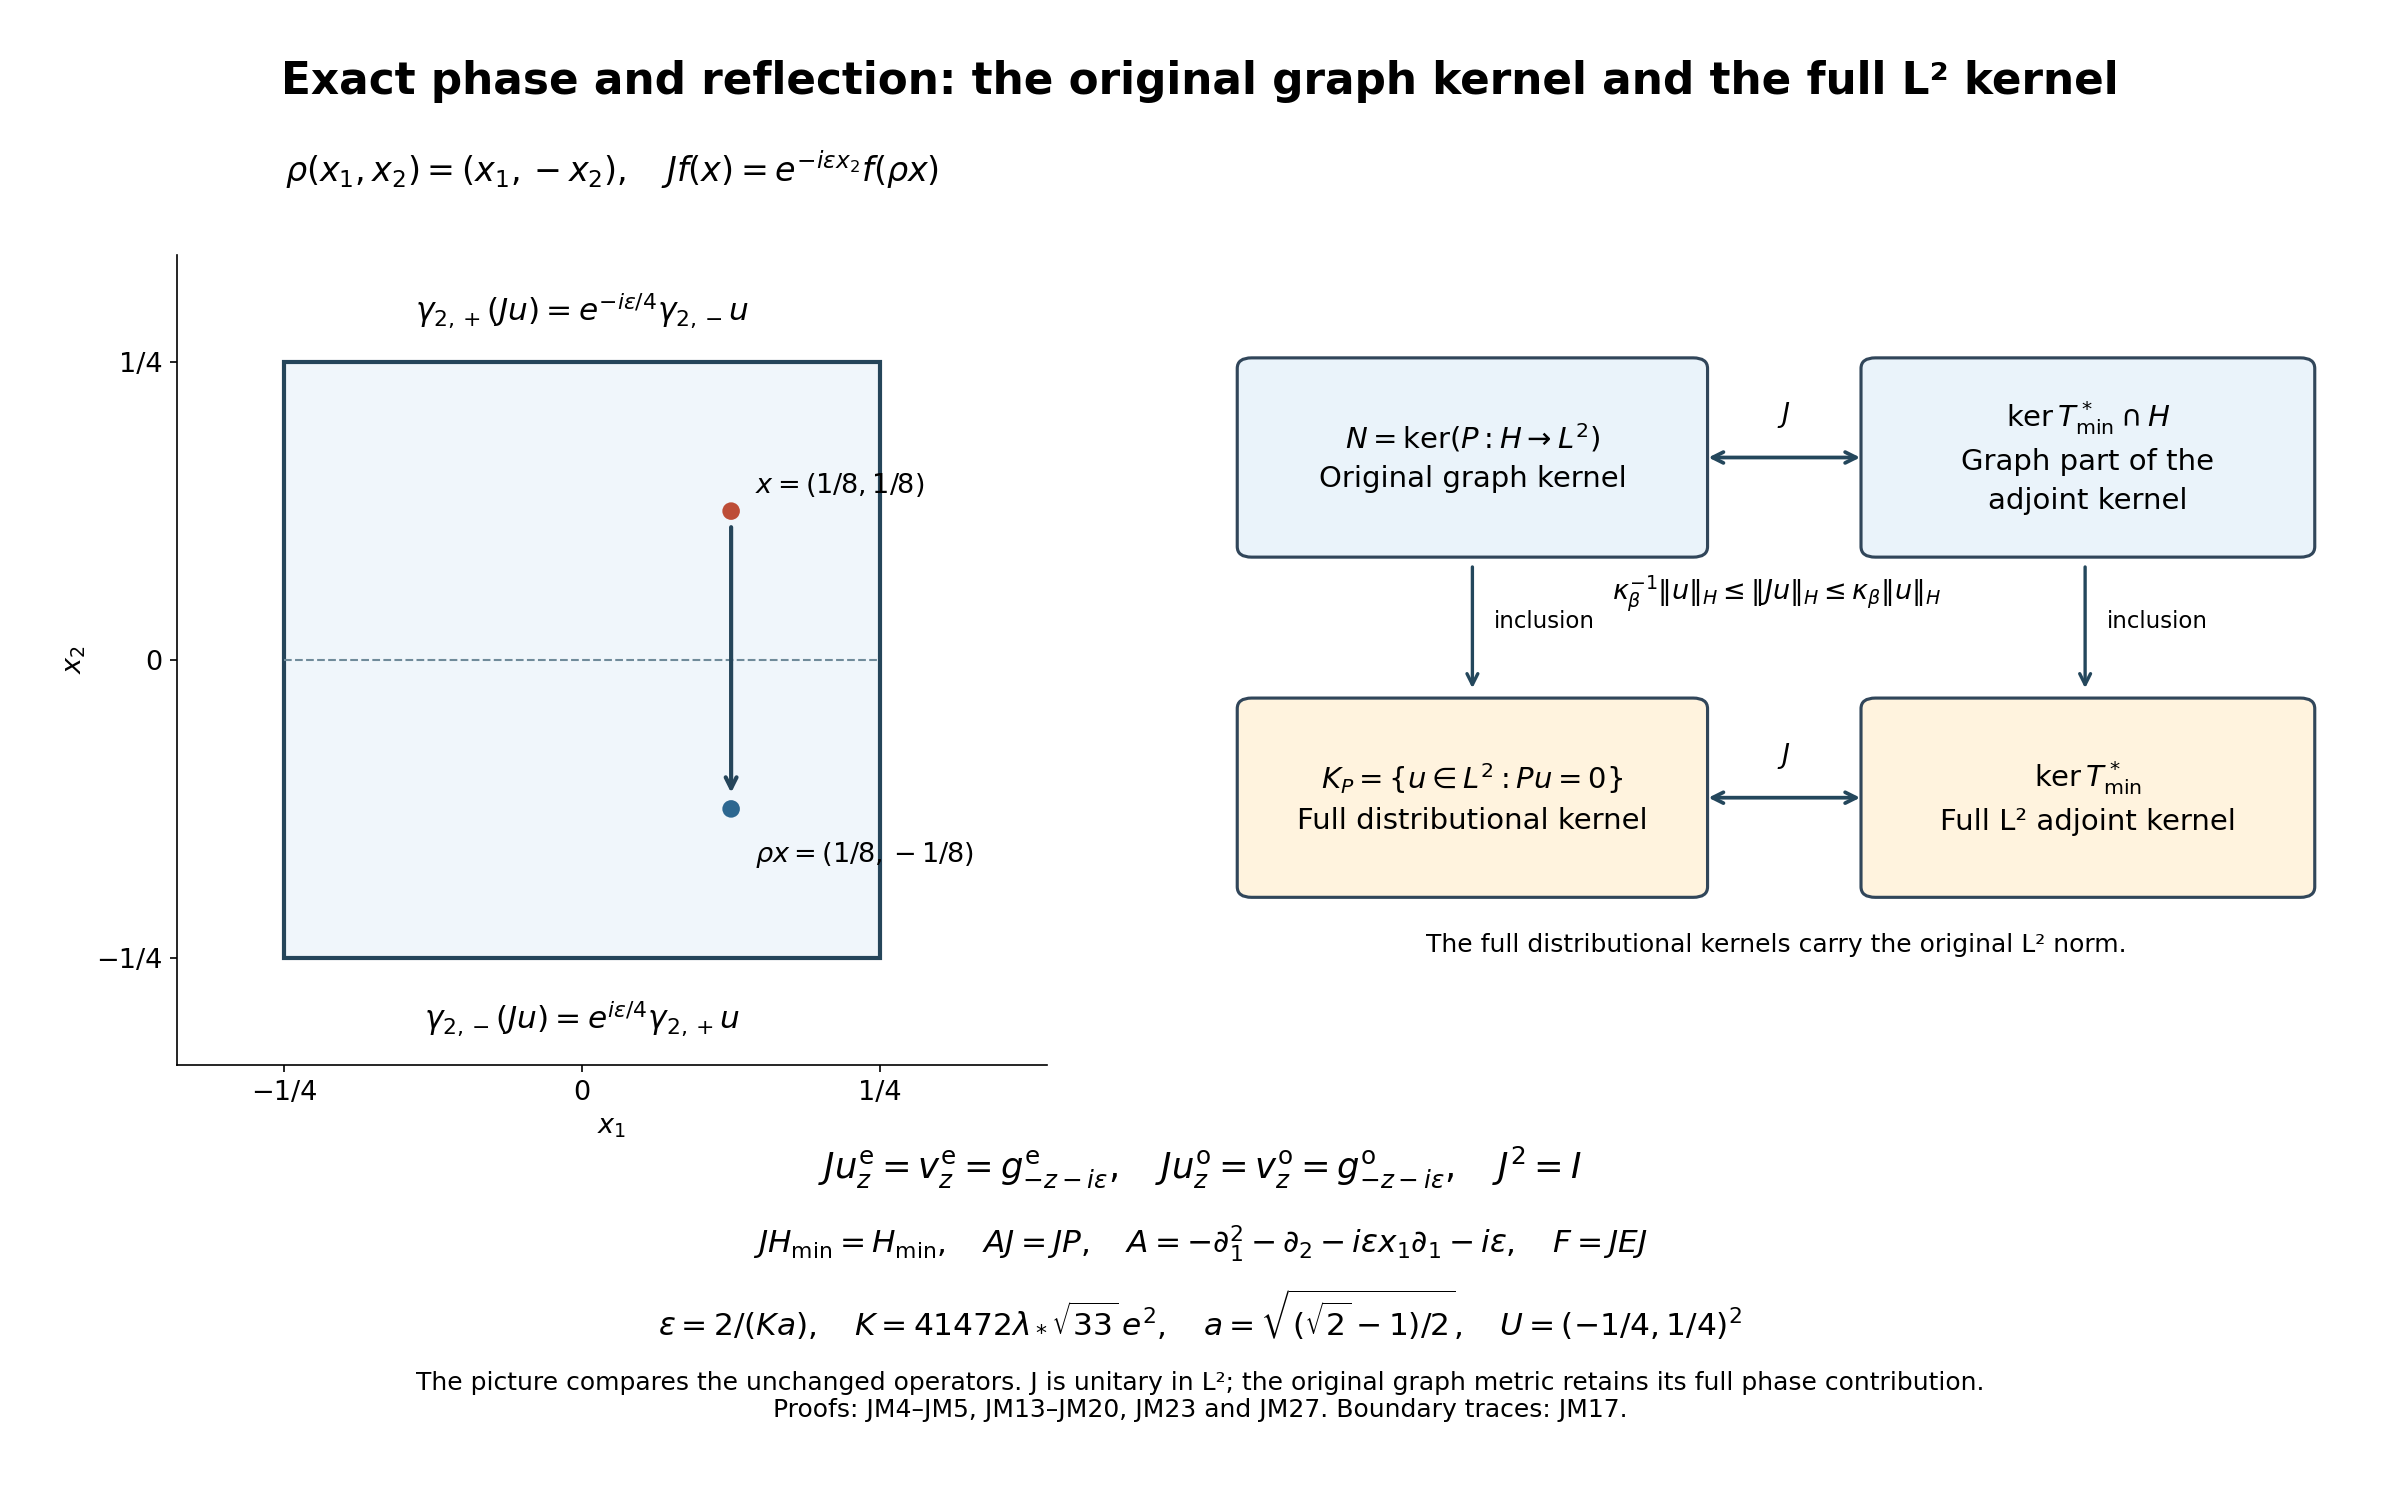
\includegraphics[width=.99\textwidth]{figures/reflection_graph_kernel_bridge.png}
\caption{The two exact kernel bridges, the full phase and reflection, and trace transport on the original square. Complete proofs: JM4--JM5, JM13--JM17 and JM19--JM20. The graph-kernel intersection is retained.}
\end{figure}

\end{document}
